\documentclass[a4paper,12pt]{report}
\usepackage{alltt, fancyvrb, url}
\usepackage{graphicx}
\usepackage[utf8]{inputenc}
\usepackage{hyperref}
\usepackage[italian]{babel}
\usepackage[italian]{cleveref}
\usepackage[margin=0.5in]{geometry}
\usepackage{scrextend}

\title{Progetto di Reti \\
\large Traccia n° 2}
\author{Christian Ricci}
\date{\today}

\begin{document}
\maketitle
\tableofcontents

\chapter{Introduzione}

Il progetto consiste in un web server fatto per uno store immaginario, basato sul gioco online \textit{Krunker.io}. Gli utenti che si connettono al sito possono: 
\begin{itemize}
\item Collezionare \textit{KR}, la moneta immaginaria del gioco;
\item Possono comprare nuove armi del gioco usando i KR;
\item Possono vedere le loro statistiche (KR e armi già comprate).
\end{itemize}

Il web server ha anche un sistema per servire pagine dinamiche, un sistema di autenticazione degli utenti e un concetto molto semplice di sessione.

\chapter{Servizi del sito}

\begin{figure}[h]
\centering{}
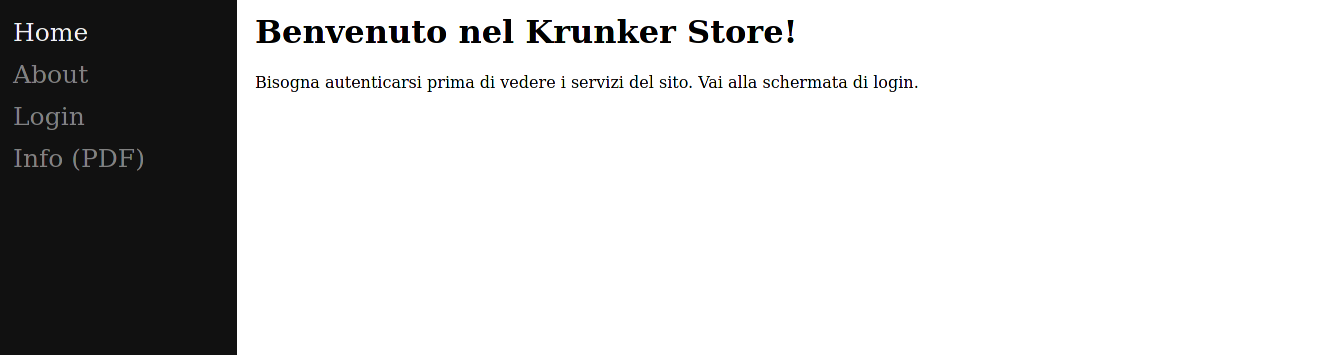
\includegraphics[width=\textwidth]{home1.png}
\caption{La schermata principale per gli ospiti.}
\label{img:home_guest}
\end{figure}

\begin{figure}[h]
\centering{}
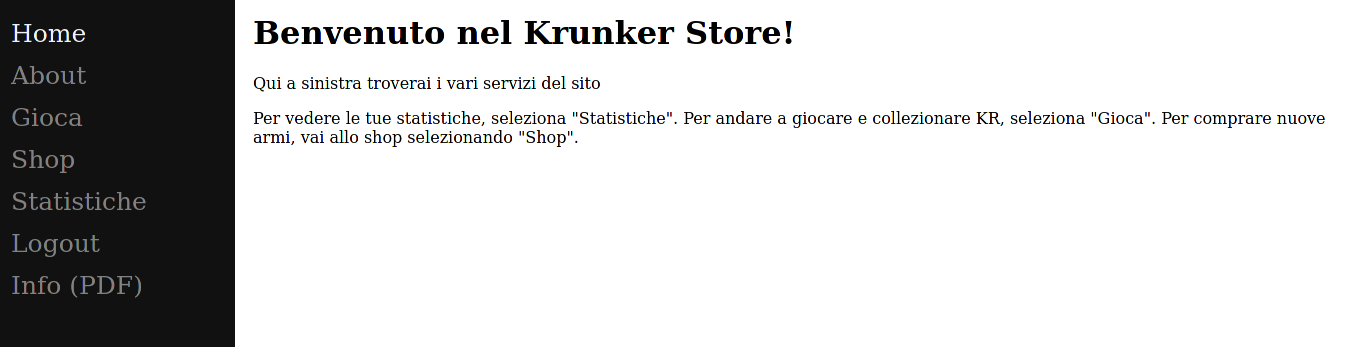
\includegraphics[width=\textwidth]{home2.png}
\caption{La schermata principale per gli utenti, che mostra anche i principali servizi del sito.}
\label{img:home_user}
\end{figure}

Prima di vedere i servizi del sito, gli utenti dovranno fare il login. I servizi che il sito mette a disposizione si possono trovare tutti nella \textit{sidebar} e sono i seguenti:
\begin{itemize}
\item Gioca: qui è dove gli utenti possono giocare e collezionare più KR. Normalmente in una pagina del genere ci dovrebbe essere un gioco completo; dato che lo scopo principale del progetto non è creare un gioco, ma bensì creare un web server, si è optato per una semplice pagina con un bottone. Il bottone manda una richiesta POST al server, in cui nel contenuto si potrà trovare il numero di KR, generato casualmente, da aggiungere al numero di KR collezionati dall'utente.
\item Shop: questo è lo \textit{store} del sito: qui gli utenti possono comprare le armi con i KR che hanno collezionato. Per ogni arma c'è un bottone apposito per comprarla: il bottone manda una richiesta POST al server, con un contenuto che sarà semplicemente l'ID dell'arma. Il server andrà a guardare se l'utente ha abbastanza KR e non ha già comprato l'arma; quindi, se è tutto andato a buon fine, scriverà in un database l'acquisto effettuato e e il nuovo ammontare di KR per l'utente.
\item Statistiche: in questa pagina ogni utente troverà le proprie statistiche, che riguardano l'ammontare di KR e le armi già comprate. Tutte queste informazioni vengono prelevate dal server ogni volta che arriva una richiesta GET per questa pagina.
\end{itemize}

Nella \textit{sidebar} si possono anche trovare un link ad un PDF con alcune informazioni sul sito e un link per le pagine di login/logout. Anche le pagine di login/logout mandano una richiesta POST al server: anche se forse per le altre pagine bastava fare una richiesta GET, per il login è necessario fare richieste POST, dato che con le GET le informazioni sulla password verrebbero messe in chiaro.

È da notare che nessuna pagina manda un nome utente nelle sue richieste al server: questo perchè il server usa l'indirizzo IP dell'utente per riconoscerlo.

\chapter{Struttura del Web Server}

Il progetto è diviso in tre moduli: un modulo per il server, un modulo per il database degli utenti e un modulo per le pagine dinamiche. Non c'è una parte di client, dato che per un web server il client di solito è il web browser dell'utente.

\begin{figure}[h]
\centering{}
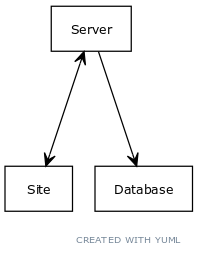
\includegraphics[]{uml1.png}
\caption{La struttura dei moduli.}
\label{img:uml_modules}
\end{figure}

\section{Server}

Il server si occupa di gestire, appunto, il server e le richieste che vengono fatte ad esso. Per il server sono state utilizzate le librerie che il linguaggio Python metteva già a disposizione:
\begin{itemize}
\item \textit{socketserver}: questa libreria implementa molte classi di server. Da qui viene la classe

\texttt{ThreadingTPCServer}, una classe che gestisce le connessioni usando più thread, permettendo l'accesso a più utenti in contemporanea.
\item \textit{http.server}: questa libreria implementa classi per server HTTP, ma anche classi per le richieste HTTP. Una di queste, la classe \texttt{SimpleHTTPRequestHandler}, è stata usata per gestire le richieste dei client.
\item \textit{cgi}: è una libreria per il supporto al Common Gateway Interface. Nel contesto del server, questa libreria è stata usata per il \textit{parsing} del contenuto delle richieste POST.
\end{itemize}

La struttura del server è molto semplice: un'istanza della classe \texttt{ThreadingTCPServer} è usata per il server vero e proprio, e fa uso di una classe StoreRequestHandler, che eredita da \texttt{SimpleHTTPRequestHandler}, per gestire le richieste. Qui di seguito uno schema delle classi.

La classe \texttt{StoreRequestHandler}, essendo il gestore delle richieste, si occupa di:
\begin{itemize}
\item Servire pagine dinamiche: questo lo fa utilizzando il modulo del sito. In generale, quando il gestore si accorge che l'utente sta chiedendo una pagina dinamica, allora creerà una nuova pagina e servirà quella.
\item Gestire le richieste POST: alcune pagine fanno richieste POST specifiche per quella pagina, ad esempio la pagina di login invia informazioni riguardanti il nome utente e la password. Il gestore, per ogni pagina che fa richieste POST, ha una funzione dedicata a gestire la richiesta.
\item Gestire i login degli utenti: questo viene fatto utilizzando una semplice tabella che memorizza indirizzo IP e nome utente. Questo approccio semplifica anche le richieste POST fatte dalle altre pagine: a queste non serve mandare un nome utente, dato che il nome utente si può subito trovare usando l'indirizzo IP. È da notare che un sistema di login così, anche se semplice, non è molto sicuro: un sistema fatto bene dovrebbe anche criptare le password.
\item Fare il log delle richieste fatte: queste vengono scritte su file di log specifici, che si possono trovare nella directory \textit{files}.
\end{itemize}

\section{Sito}

Il modulo del sito si occupa di gestire i contenuti, dinamici e non, del sito, che significa quindi:

\begin{itemize}
\item Prelevare i contenuti delle pagine dai loro file \textit{template} (contenuti tutti in una cartella denominata "templates");
\item A richiesta, creare una pagina dinamica per un utente specifico o per un ospite del sito;
\item Manipolare le pagine statiche del sito;
\end{itemize}

A questo scopo definire una classe \texttt{Page} ed una tabella di pagine per definire quali sono le pagine dinamiche del sito, e offre alcune funzioni per manipolare le suddette pagine.

Una \texttt{Page} rappresenta una pagina dinamica. Al momento della creazione, un'instanza di \texttt{Page} legge dal proprio file i suoi contenuti: così facendo non si dovrà sempre andare a leggere il file in sè. Ogni pagina definire anche un livello di accesso: Solo Ospite, Solo Utente o tutti e due. Questa proprietà è usata, per esempio, per negare l'accesso ai client ospiti alle pagine che solo gli utenti dovrebbero accedere. Infine, una \texttt{Page} può avere una versione per gli ospiti e per gli utenti.

Per creare una pagina dinamica, basta usare la funzione \texttt{create\_page}, che andrà a creare una nuova pagina basandosi su un url e un nome utente e andrà a scriverla nella directory di root del sito.

Ad una pagina si può aggiungere altri contenuti dinamici: ad esempio, con la funzione \texttt{page\_on\_GET}, a cui si passa una funzione, ogni volta che verrà fatta una richiesta GET di una pagina, a questa verrà aggiunto altro contenuto definito dalla funzione passata.

Infine, un'altra funziona, chiamata \texttt{load\_page\_cached}, viene usata per caricare più velocemente alcune pagine statiche. La funzione usa una cache propria per contenere le pagine caricate.

\section{Database}

Il modulo del database implementa un database molto semplice per gli utenti e i loro dati.

L'approccio che si è utilizzato è di usare un file per contenere i dati degli utenti, che viene letto quando il server viene fatto partire, e viene scritto sia quando viene fatto un aggiornamento alla struttura dati nel programma, sia quando il server viene chiuso. La struttura dati per il database è una semplice classe, chiamata \texttt{UserDatabase}, che eredita da una classe built-in di Python, \texttt{dict}, e che offre un metodo per salvare il database su file. Il database quindi opera come un dizionario.

Nel modulo del database si possono anche trovare informazioni sulle armi. Dato che queste informazioni sono read-only, non c'è bisogno di avere una gestione avanzata e quindi si è optato per un semplice array.

\begin{figure}[h]
\centering{}
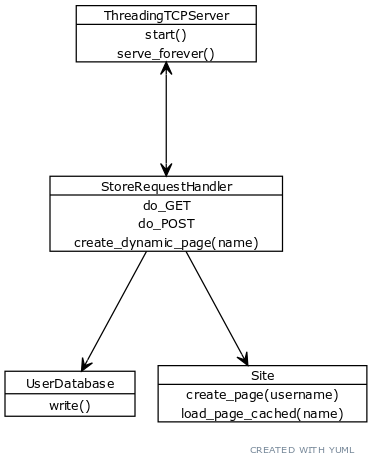
\includegraphics[]{uml2.png}
\caption{La struttura finale del progetto.}
\label{img:uml_classes}
\end{figure}

\end{document}